\documentclass[11pt,a4paper]{article}
\usepackage[utf8]{inputenc}
\usepackage[T1]{fontenc}
\usepackage{lmodern}
\usepackage{textcomp}
\input{glyphtounicode}
\pdfgentounicode=1
\usepackage{amsmath,amssymb}
\usepackage{microtype}
\usepackage{graphicx}
\usepackage{booktabs}
\usepackage[margin=1in]{geometry}
\usepackage{natbib}
\usepackage{float}
\usepackage{hyperref}
\hypersetup{colorlinks=true,allcolors=black,
  pdftitle={Correcting Fund Performance Rankings Under Regime Difficulty with Item Response Theory},
  pdfauthor={Jung Min Kang},
  pdfkeywords={Item Response Theory, Fund Evaluation, Market Regimes, EFSL}}

\title{Correcting Fund Performance Rankings Under Regime Difficulty\\with Item Response Theory}
\author{Jung Min Kang\\\textit{Independent Researcher, Seoul, South Korea}\\\texttt{gangjeongmin23@gmail.com}\\ORCID: 0009-0007-9599-2792}
\date{May 2026}

\begin{document}
\maketitle

\begin{abstract}
We apply the Evaluation Failure Scaling Law (EFSL) framework to global fund performance assessment, showing that simple averaging of binary monthly outperformance can produce substantial model-implied ranking distortions under regime-dependent period difficulty. Using a 2-parameter logistic Item Response Theory (IRT) model on 50 exchange-traded funds across 217 monthly periods (April 2008 to April 2026), we find that IRT corrections shift fund rankings by up to $\pm$30 positions (Spearman $\rho = 0.573$). Crisis periods exhibit lower IRT difficulty than normal periods (month-level Mann--Whitney $p = 0.001$; contiguous-block permutation $p = 0.055$), consistent with the interpretation that market downturns are easier periods for relative outperformance. The Linear Logistic Test Model provides an exploratory decomposition of period difficulty, though cross-validated performance is weak ($R^2_{\text{CV}} < 0$). Principal Component Regression indicates a dominant common return component (PC1 = 59.2\%). A sparsity stress test with a 1PL Rasch refit compares rankings under artificial masking against the full-data 2PL ranking, which is itself an IRT estimate rather than an external ground truth. The canonical run recorded the 1PL refit ahead of simple averaging at 7 of 10 sparsity levels (0--90\%, including the unmasked level), but its per-level values were not committed; an offline refit gives 6 of 10, with IRT advantages of $+0.003$ to $+0.014$ in Spearman $\rho$ and losses at 50\%, 70\%, 80\%, and 90\% sparsity (down to $-0.041$ at 90\%). This provides an additional cross-domain application of the EFSL framework.

\medskip\noindent\textbf{Keywords:} Item Response Theory, Fund Evaluation, Market Regimes, EFSL
\end{abstract}

\section{Introduction}

Fund performance evaluation relies on simple average returns, Sharpe ratios, and Jensen's alpha \citep{sharpe1966,jensen1968}. These methods assume all evaluation periods contribute equally---an assumption that fails when funds operate across market regimes of varying difficulty and not all funds exist in all periods.

The Evaluation Failure Scaling Law \citep{kang2026efsl} demonstrates that simple averaging produces unreliable rankings under high sparsity and heterogeneous item difficulty. We extend this framework to finance with the structural mapping: subjects ($\theta$) = 50 global ETFs; items ($b$) = 217 monthly periods; binary response = did the fund beat ACWI in that month? Because most ETFs in our universe are passive index trackers rather than actively managed funds, the latent ``fund ability'' parameter $\theta$ should be interpreted as a benchmark-relative outperformance propensity driven by asset-class exposure, not as a measure of active management skill.

We apply three tools: (1)~IRT (2PL) to jointly estimate fund ability and period difficulty with post-optimization centering; (2)~LLTM to explore whether macro features explain period difficulty; (3)~PCR to extract latent market factors.

\section{Data and Methods}

\subsection{Data}

Daily adjusted closing prices for 50 U.S.-listed ETFs and the MSCI ACWI ETF benchmark are collected via Yahoo Finance. The sample begins April 2008, after the ACWI ETF's launch date of March 26, 2008, to ensure a consistent benchmark throughout. The sample ends April 2026, yielding 217 monthly periods.

\begin{table}[H]
\centering\small
\caption{ETF universe by region.}
\label{tab:universe}
\begin{tabular}{@{}lrl@{}}
\toprule
\textbf{Region/Class} & \textbf{N} & \textbf{Examples} \\
\midrule
US Broad \& Growth   & 7  & SPY, QQQ, IWM, DIA, ARKK, VTI, VOO \\
US Sectors           & 11 & XLK, XLF, XLE, XLV, XLRE, SMH, XLU, XLI, XLP, XLB, XLC \\
Europe               & 9  & EWG, EWU, EWQ, EWI, EWP, EWL, EWN, EWD, EWK \\
Asia-Pacific         & 7  & EWJ, EWY, EWA, EWT, EWS, EWH, MCHI \\
Emerging Markets     & 8  & EEM, EWZ, INDA, EWW, TUR, EZA, ECH, EPOL \\
Commodities/Crypto   & 3  & GLD, SLV, IBIT \\
Fixed Income/REITs   & 5  & TLT, HYG, LQD, TIP, VNQ \\
\midrule
\textbf{Total}       & \textbf{50} & \\
\bottomrule
\end{tabular}
\end{table}

The binary response matrix has 10,233 observed entries out of 10,850 possible (94.3\% coverage, 5.7\% natural sparsity). Missing entries arise when funds did not yet exist (e.g., IBIT launched January 2024).

\paragraph{Data availability.} Raw price data is sourced from Yahoo Finance via the \texttt{yfinance} Python library, which is intended for personal and research use. We provide exact tickers and date ranges in a manifest file; users must download data themselves. This study is for research purposes only and does not constitute investment advice. Yahoo Finance data are informational and may be revised; users should verify data independently.

\subsection{IRT (2PL) Model}

We fit a 2-parameter logistic IRT model:
$P(X_{ij}=1 \mid \theta_i, a_j, b_j) = [1+\exp(-a_j(\theta_i - b_j))]^{-1}$,
where $\theta_i$ is fund ability, $b_j$ is period difficulty, and $a_j > 0$ is discrimination. Parameters are estimated by L-BFGS-B with analytic gradients.

\paragraph{Identification.} The 2PL likelihood is invariant to a joint location shift of $\theta$ and $b$. We resolve this indeterminacy by post-optimization centering: $\theta_i \leftarrow \theta_i - \bar{\theta}$ and $b_j \leftarrow b_j - \bar{b}$. Scale is controlled operationally by bounding log-discrimination parameters ($|\log a_j| \leq 5$). All rank-based fund comparisons and period-difficulty comparisons are invariant to this additive centering; absolute parameter magnitudes should not be over-interpreted.

\paragraph{Assumptions.} IRT assumes unidimensionality, local independence, and monotonicity. In finance, unidimensionality is approximate: a single ``ability to outperform'' dimension captures most variance but ignores multi-factor style exposures. Local independence is violated by temporal autocorrelation between adjacent months within the same market regime. We partially address this via the contiguous-block permutation test (Section~3.2). Formal goodness-of-fit diagnostics (e.g., $Q_3$ statistics for residual dependence) are deferred to future work.

\subsection{LLTM, PCR, and Crisis Validation}

The LLTM decomposes $b_j = \sum_f q_{jf} \eta_f + \epsilon_j$ using 5 features (VIX, dispersion, ACWI return, credit spread, crisis flag) via Ridge regression with 10-fold CV.

PCA is applied to the standardized return matrix; the first $k$ components predict IRT difficulty via OLS.

Seven known crises serve as external validation. Because adjacent crisis months are autocorrelated, we supplement the month-level Mann--Whitney test with a \textbf{contiguous-block permutation test}: for each of the 7 crisis episodes, we compute the mean $b$ across its months, then repeatedly sample contiguous blocks of the same length from the full time series (10,000 permutations), comparing the observed crisis-episode mean against the null distribution.

\section{Results}

\subsection{IRT Ranking Corrections}

The 2PL model converges in 740 iterations. Spearman $\rho = 0.573$ ($p < 10^{-4}$), Kendall $\tau = 0.402$ ($p < 10^{-4}$). The maximum rank shift is $\pm$30 positions.

Fixed-income funds are the most upgraded: long-term bonds (TLT) shift $+$30 positions, high-yield bonds (HYG) $+$28, and investment-grade bonds (LQD) $+$24.5. European equities receive the largest downgrades: Italy (EWI) shifts $-$30, Spain (EWP) $-$29 (Figure~\ref{fig:rank}).

Regional corrections are systematic: US-region funds (incl.\ bonds/REITs) receive moderate corrections (mean $|\Delta| = 8.8$, $n = 23$), European funds the largest (mean $|\Delta| = 14.9$, $n = 9$), followed by emerging markets ($9.8$, $n = 8$) and Asia-Pacific ($7.4$, $n = 7$).

\begin{figure}[H]
\centering
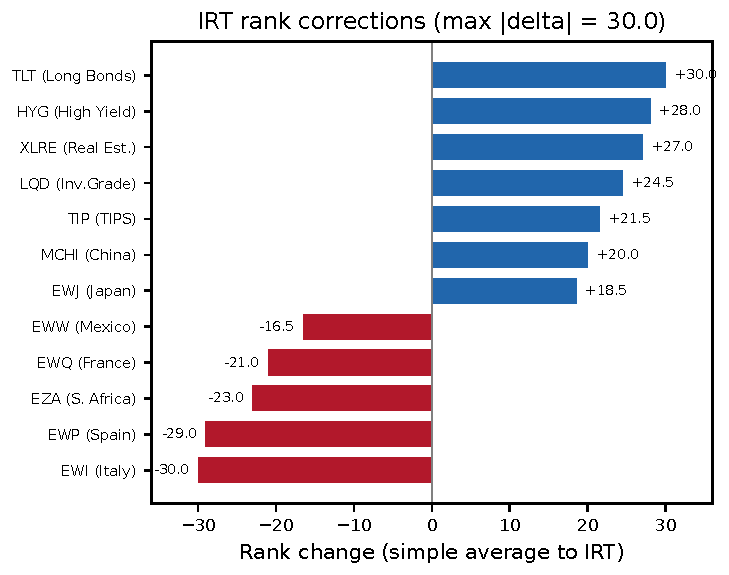
\includegraphics[width=0.85\textwidth]{figures/fig1_rank_corrections.pdf}
\caption{IRT rank corrections for the 12 largest movers. TLT ($+$30) and HYG ($+$28) are the most upgraded; EWI ($-$30) and EWP ($-$29) the most downgraded.}
\label{fig:rank}
\end{figure}

\subsection{Crisis Cross-Validation}

Crisis periods have mean $b = -0.710$; normal periods have mean $b = 0.141$. The month-level Mann--Whitney test gives $p = 0.001$. The contiguous-block permutation test gives $p = 0.055$---marginal at $\alpha = 0.05$, consistent with but not conclusively confirming a difficulty difference after accounting for temporal dependence (Figure~\ref{fig:crisis}).

The negative crisis difficulty is consistent with the interpretation that downturns are easier for relative outperformance: when ACWI drops, bonds, gold, and defensive sectors mechanically outperform. The beat rate--difficulty correlation is $r = -0.733$ ($p < 10^{-6}$), providing suggestive construct-validity evidence.

\begin{figure}[H]
\centering
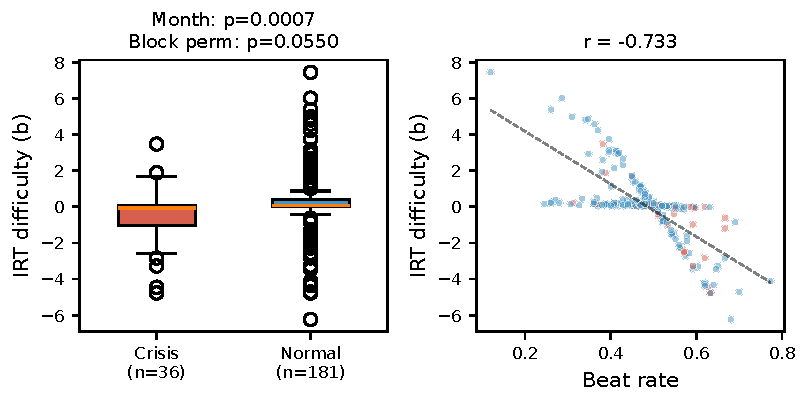
\includegraphics[width=0.85\textwidth]{figures/fig2_crisis_validation.pdf}
\caption{Left: difficulty by crisis status (month $p = 0.001$; block permutation $p = 0.055$). Right: beat rate vs.\ difficulty ($r = -0.733$). Red = crisis.}
\label{fig:crisis}
\end{figure}

\subsection{LLTM Decomposition}

The LLTM achieves in-sample $R^2 = 0.076$ but cross-validated $R^2 = -0.048 \pm 0.190$, indicating that the 5-feature linear model does not reliably predict out-of-sample monthly difficulty. Feature weights are exploratory: ACWI return ($\eta = +0.25$), credit spread ($\eta = -0.22$), crisis flag ($\eta = -0.18$), and dispersion ($\eta = -0.17$). These should not be treated as confirmatory (Figure~\ref{fig:lltm}).

\begin{figure}[H]
\centering
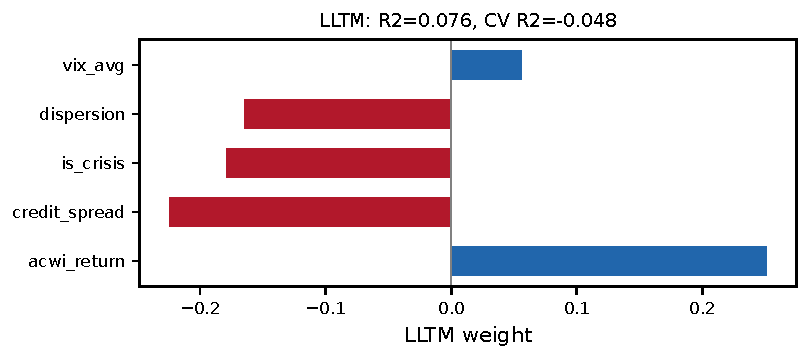
\includegraphics[width=0.85\textwidth]{figures/fig3_lltm_weights.pdf}
\caption{LLTM feature weights (exploratory). Cross-validated $R^2 < 0$.}
\label{fig:lltm}
\end{figure}

\subsection{PCR Factor Structure}

PC1 explains 59.2\% of variance, consistent with a dominant common return component, with top-3 PCs at 70.9\% (Figure~\ref{fig:pca}). PCR with 3 components predicts difficulty at $R^2 = 0.104$.

\begin{figure}[H]
\centering
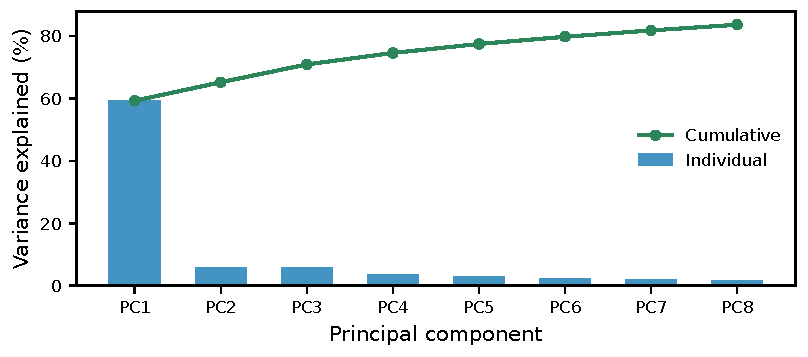
\includegraphics[width=0.85\textwidth]{figures/fig4_pca_variance.pdf}
\caption{PCA variance explained.}
\label{fig:pca}
\end{figure}

\subsection{Sparsity Stress Test}

We randomly mask a fraction $s \in \{0, 0.1, \dots, 0.9\}$ of the observed entries, refit a 1PL Rasch model for computational stability, and compare the Spearman $\rho$ of the 1PL and simple-average rankings against the full-data 2PL ranking. This reference ranking is the main IRT estimate, not an external ground truth, so the test measures agreement with the full-data IRT solution; the $s = 0$ level applies no masking and is counted as one of the 10 levels. The canonical run (\texttt{experiment.py}: 5 masking replicates per level, L-BFGS-B \texttt{maxiter} 300) recorded the 1PL refit ahead at 7 of 10 levels (Figure~\ref{fig:stress}); only this count, not the per-level values, is committed as data (\nolinkurl{data/canonical_stress.json}). An offline refit (\nolinkurl{reproduce_from_derived.py} \texttt{-{}-stress-refit}: 2 masking replicates per level, \texttt{maxiter} 200; per-level values in \nolinkurl{data/stress_refit_levels.csv}) gives 6 of 10: the 1PL refit leads by $+0.003$ to $+0.014$ at $s = 0$--$0.4$ and $s = 0.6$, and trails at $s = 0.5$ ($-0.002$), $0.7$ ($-0.002$), $0.8$ ($-0.017$), and $0.9$ ($-0.041$). IRT therefore loses at high sparsity in the offline refit. We note that the stress-test refit uses a simpler model than the main 2PL analysis; the 1PL omits discrimination parameters, providing a lower-capacity robustness check rather than an exact replication of the main 2PL estimator.

\begin{figure}[H]
\centering
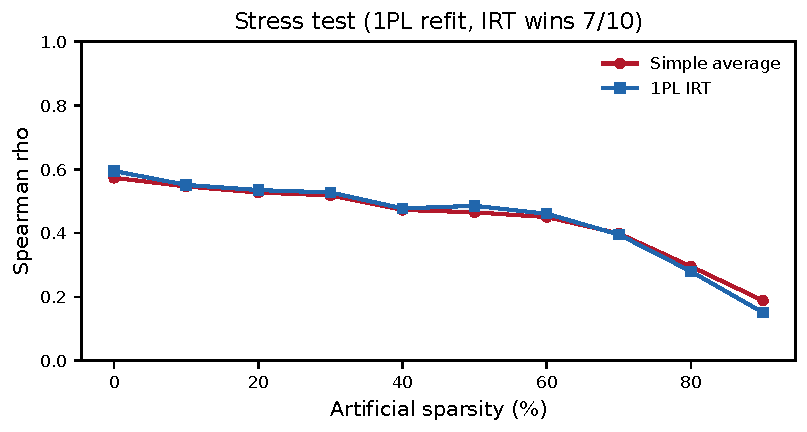
\includegraphics[width=0.85\textwidth]{figures/fig5_stress_test.pdf}
\caption{Sparsity stress test using 1PL Rasch refit, canonical run (recorded as 7/10 IRT wins; per-level values not committed as data). Reference ranking: full-data 2PL estimate. The offline refit (6/10; \nolinkurl{data/stress_refit_levels.csv}) is reported in the text.}
\label{fig:stress}
\end{figure}

\subsection{Regional Analysis}

European funds receive the largest corrections (mean $|\Delta| = 14.9$), followed by emerging markets ($9.8$). Asia-Pacific ($7.4$) and global/commodity funds ($4.7$) receive smaller corrections than US-region funds (incl.\ bonds/REITs; $8.8$) (Figure~\ref{fig:regions}).

\begin{figure}[H]
\centering
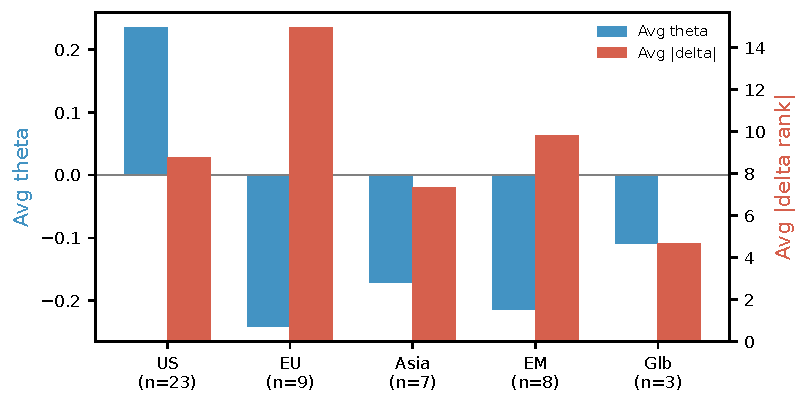
\includegraphics[width=0.85\textwidth]{figures/fig6_regions.pdf}
\caption{IRT ability and correction magnitude by region.}
\label{fig:regions}
\end{figure}

\section{Discussion}

\paragraph{Difficulty inversion.} Crisis periods appear easier for relative outperformance, consistent with the EFSL pattern where ``hard'' conditions for observers differ from ``hard'' conditions for the ranking problem. However, the block-level permutation ($p = 0.055$) indicates this difference is marginal once temporal autocorrelation is accounted for; future work with more crisis episodes or longer history may clarify this.

\paragraph{Comparison to risk-adjusted metrics.} Sharpe ratios and factor alphas \citep{sharpe1966,jensen1968,fama1993common,carhart1997persistence} assess whether funds generate excess risk-adjusted return. IRT assesses whether a fund's \textit{ranking} is distorted by regime-specific evaluation bias. The two are complementary. Future work should examine whether IRT-corrected rankings predict out-of-sample performance better than factor-based rankings.

\paragraph{Limitations.} Unidimensionality and local independence are approximate; formal diagnostics are needed. Because the universe mixes equity, fixed-income, commodity, real-estate, and digital-asset ETFs, estimated period difficulty partly reflects benchmark-relative asset-class exposure rather than a pure market-regime difficulty parameter; crisis ``easiness'' is partly mechanical when non-equity assets are compared against an equity benchmark. LLTM does not generalize out-of-sample at monthly resolution. The stress test uses a simpler 1PL model. Natural sparsity (5.7\%) is low compared to other EFSL domains.

\section{Conclusion}

IRT rank corrections of $\pm$30 positions among 50 global ETFs suggest that regime-dependent evaluation effects can materially alter fund rankings. Crisis periods are consistent with being easier for relative outperformance (block permutation $p = 0.055$). In the sparsity stress test (1PL, scored against the full-data IRT ranking), the canonical run recorded IRT ahead at 7/10 levels without committed per-level values, while an offline refit gives 6/10 with margins of at most $+0.014$ and losses at high sparsity (down to $-0.041$ at 90\%). This provides an additional cross-domain application of the EFSL framework.

Code and reproduction artifacts are provided in the accompanying source package.

\bibliographystyle{plainnat}
\bibliography{references}

\end{document}
